\documentclass{report}
\usepackage{amsmath}
\usepackage{geometry}
\usepackage{graphicx}
\begin{document} 

\begin{flushleft}

\begin{Large}

\textbf{Name - Ankush Vijay Israney} \\
\textbf{Student ID - 14057308} \\
\textbf{CS 613 - Extra Credit Assignment report} \\ 

\end{Large} 

\break

\underline { \textbf{HIDDEN MARKOV MODELS}}
\section{\underline{part1 A}} 

 \begin{equation}
 P(O \mid \lambda) = 1.9153e^{-10} 
 \end{equation}
 
 \begin{equation}
 P(O \mid random) = (1/3)^{20} = 2.81115e^{-10} 
 \end{equation}
 
 \break

\section{\underline{part1 B}}

\begin{figure}[ht!]
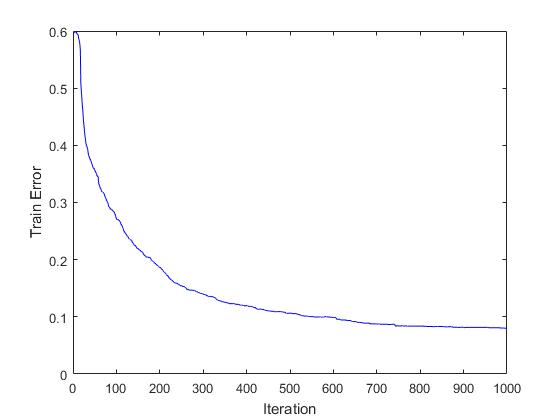
\includegraphics{part1.jpg}
\end{figure} 

\break

\section{\underline{part1 C}}

\[
\lambda = ([1 , 0], \begin{bmatrix}
0.690119 &&	0.309880 \\
0.093321	&& 0.906678 \\
\end{bmatrix}
,  \begin{bmatrix}
0.581589 && 1.211885e-08	&& 0.418410 \\
4.885295e-31	&& 0.762061   &&	0.237938 \\
\end{bmatrix}]
\]




\end{flushleft} 

\end{document}